\section{Empirical Evaluation}
\label{section:evaluation}
Please showcase your empirical results in this section. Please clearly specify which sets of experiments of the original paper are considered in your report. Please also report the corresponding hyperparameters of each experiment.

\textbf{taxi domain:}

Sarsa with epsilon-greedy, learning rate $\alpha = 0.1$, discount factor $\gamma = 1 $, we test different $\epsilon$ values, $\epsilon = 0.05, 0.1, 0.2, 0.3, 0.5$, and the result are averaged over 6 independent runs, each consisting of 100000 time steps.

Sarsa with Boltzmann softmax, learning rate $\alpha = 0.1$, discount factor $\gamma = 1 $, we test different $\beta$ values, $\beta = 0.5, 1, 2, 3, 5, 10$, and the result are averaged over 6 independent runs, each consisting of 100000 time steps.

Sarsa with Mellowmax softmax, learning rate $\alpha = 0.1$, discount factor $\gamma = 1 $, we test different $\omega$ values, $\omega = 0.5, 1, 2, 3, 5, 50$, and the result are averaged over 6 independent runs, each consisting of 10000 time steps. We know that when $\omega \to \infty$, Mellowmax will behave like max operator, and we set $\omega$ to 50 so that the result will similar to the paper and show that phenomenon.

\begin{figure}[H]
\centering  
\subfigure[$\epsilon$-greedy]{
	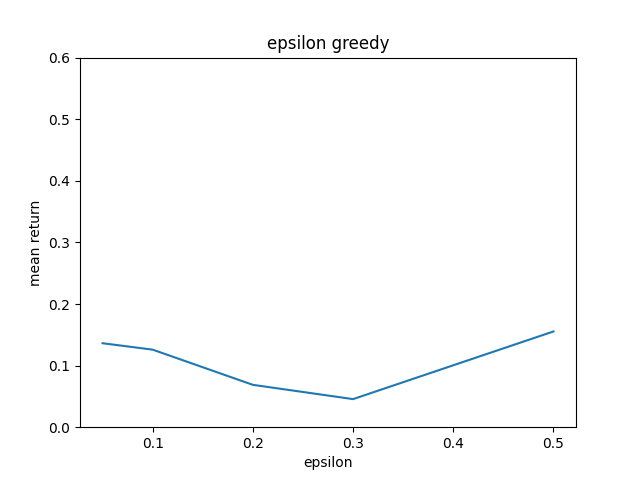
\includegraphics[width=0.3\textwidth]{taxi_1.png}}
\subfigure[Boltzmann softmax]{
	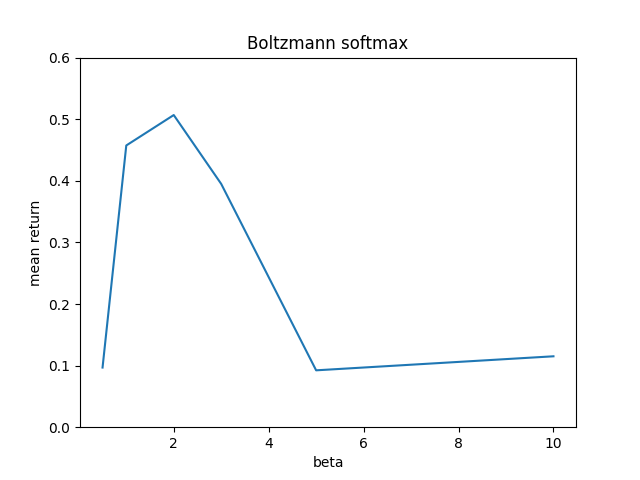
\includegraphics[width=0.3\textwidth]{taxi_2.png}}
\subfigure[Mellowmax softmax]{
	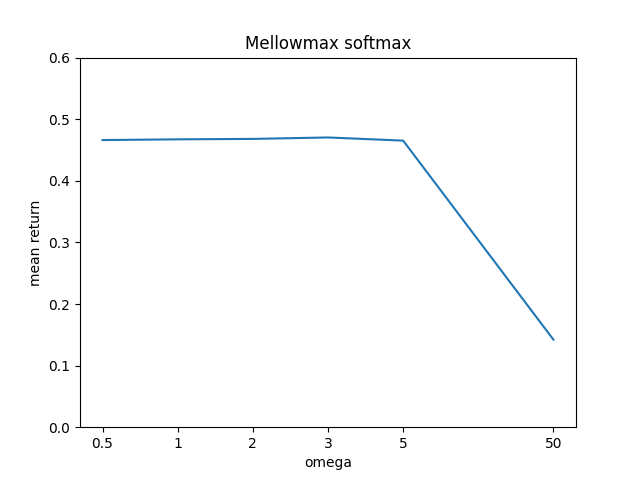
\includegraphics[width=0.3\textwidth]{taxi_3.png}}
\caption{Taxi domain result}
\end{figure}